\section{\pads{} and the Original \learnpads{}} 
\label{sec:review}

\begin{figure*}[th]
{\small \begin{verbatim}
207.136.97.49 - - [15/Oct/1997:18:46:52 -0700] "GET /turkey/back.gif HTTP/1.0" 200 224
ppp31.igc.org - amnesty [16/Oct/1997:08:40:11 -0700] "GET /members/afr.html HTTP/1.0" 200 450
\end{verbatim}                  
}
\caption{A fragment from a web server log in \ai{} format}\label{fig:ai}
\end{figure*}

This section gives an overview of the \pads{} language and the original \learnpads{}
format inference system. Figure \ref{fig:ai} shows a fragment of a web server
log. We shall call the data format 
in this log file \ai{} from now onwards. A quick analysis of the fragment reveals
that the \ai{} format is made up of a sequence of records, separated by newlines.
Each record consists of a number of fields delimited by white spaces. For example
the first record starts with an IP address, then two dashes, a time stamp enclosed in
a pair of square brackets, followed by a quoted HTTP message and two integers.
The format varies slightly in the second the the third record. In particular,
the IP address becomes a hostname and the second dash becomes an English word 
(or an identifier) in the second line. 

\begin{figure}[t]
{\small \begin{verbatim}
Punion client_t {
  Pip       ip;      // 207.136.97.49
  Phostname host;    // ppp31.igc.org 
};
Punion auth_id_t {
  Pchar unauthorized : unauthorized == '-'; 
  Pstring id;                        
};
Pstruct request_t {
   "\"GET ";    Ppath    path;
   " HTTP/";    Pfloat   http_ver; 
   '\"'
}
Pstruct entry_t {
         client_t       client;          
   ' ';  auth_id_t      remoteID;        
   ' ';  auth_id_t      auth;            
   " ["; Pdate          date;   
   ':';  Ptime          time;     
   "] "; request_t      request;         
   ' ';  Pint           response;     
   ' ';  Pint           length; 
};
\end{verbatim}
}
\caption{\padsc{} description for the \ai{} format}
\label{fig:ai.p}
\end{figure}

Figure \ref{fig:ai.p} shows the \padsc {} description of {\em any}
of the two records in Figure \ref{fig:ai}. \padsc{} is a variant of the
\pads{} language which follows C syntax closely. 
The \pads{} is a data description language based on programming language types 
\cite{sigcomm00,gpce02}. 
Types are interpretated as grammars and are used to describe data structures.
A \padsc{} description consists of a series declarations. Each declaration
has a keyword such as ``Pstruct'', a name for the type such as ``entry\_t'',
and the actual definition block of the type, which typically is a series of
fields separated by semicolons. The ``Pstruct'' keyword indicates the type
is a sequence of structure, each represented by a field in the definition.
The ``Punion'' keyword means the type is a union of a number of choices,
each again represented by a field in the definition. Each field is either
a constant string, or a type name followed by a variable name. The variable
name can be used to refer to the field. In addition to complex types
like structs and unions, \padsc{} also 
offers a variety of base types such as {\tt Pint}, {\tt Pip} and {\tt Ptime},
each of which represent a basic data type such as integer, IP address and
time. The \pads{} language also has other features
such as constraints and dependencies which are not illustrated in the example
above. 

%Each record in Figure \ref{fig:ai} can be defined by a Pstruct type called \verb#entry_t#, 
%and is denoted as a record by the {\tt Precord} keyword. 
%The first field in \verb#entry_t# is defined by a type called 
%\verb#client_t#, which itself is a union of two base types, a Pip and
%a Phostname. The second and third field can be described by a type
%called \verb#auth_id_t#, which is another union of two base types.
%Finally the HTTP request message can be described by a struct type
%called \verb#request_t#. 

The goal of the \learnpads{} format inference engine is to 
learn a \pads{} description like in Figure \ref{fig:ai.p} from
the raw data itself and produce end-to-end processing tools fully
automatically. \learnpads{} achieves this through a three-phase algorithm.
In the first phase ({\em tokenization}), each line of data string (a unit of
repetition) is converted into a sequences base tokens. The sequences of
tokens (shown in brackets) converted from the two example lines 
in Figure \ref{fig:ai} are:

{\small
\begin{verbatim}
[ip] [ ] [-] [ ] [-] [ ] [[] [date] [:] 
   [time] []] [ ] ["] [str] [ ] [path] [ ] 
   [str] [/] [float] ["] [ ] [int] [ ] [int]

[host] [ ] [-] [ ] [str] [ ] [[] [date] [:] 
   [time] []] [ ] ["] [str] [ ] [path] [ ] 
   [str] [/] [float] ["] [ ] [int] [ ] [int]
\end{verbatim}
}

In the second phase ({\em structure discovery}), 
a divide-and-conquer algorithm  construct a candidate description.
The algorithm computes frequency histogram for each token type in the
tokenized data from phase one. Each bar in the histogram represents
the percentage of lines that have a certain number of occurrence of
a particular token. 
%For the above tokenized data, the histograms for 
%[ip], [-] and [int] are shown in Figure \ref{fig:histograms} as an example.
%\begin{figure}[th]
%\begin{center}
%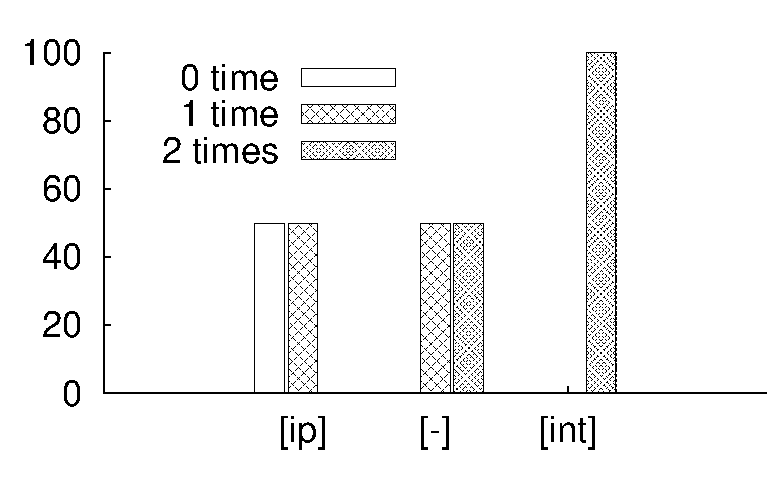
\epsfig{file=histogram1-2.eps, width=0.7\columnwidth}
%\caption{Histogram for [ip], [-] and [int]}
%\label{fig:histograms}
%\end{center}
%\end{figure}
%
The algorithm then groups the tokens by the similarity of their histograms,
and selects a group of tokens that exhibits the strongest signal of being
either struct, union or array separators. These tokens are used 
to partition the tokens into sub-contexts. For each of the sub-context,
we repeat the above procedure of computing histograms and grouping
tokens, etc in a recursive manner. At the end of phase two, we will have
a relatively good candidate structure that describes the original data records.

In the third and last phase ({\em format refinement}),
we improve the candidate structure through the application of a series of
rewriting rules. The rewriting rules are aimed at minimizing the size
of the description while
making it more precise and accurate by transforming the structures and 
adding data dependencies among sub-structures and constraints on base types.
The procedure is a greedy local search process which optimizes an information-theoretic
scoring function. 
%We pick the cost of transmitting the data and the description as our
%scoring function, following the Minimum Description Length (MDL) \cite{mdlbook} 
%principle. The phase stops when the search reaches a local optimal description.

While the above inference algorithm produces some good results for the
set of small log files that we experimented with, it has some serious
limitations. First, the algorithm requires loading all the data into main
memory at once to analyze it. This means it cannot learn the format for a log
file that is larger than the size of the usable memory. To make matters worse, the
data dependency analysis in the format refinement phase uses quadratic space. 
Therefore the algorithm simply cannot scale to real-world
system logs which are easily a few hundred megabytes to several gigabytes. 
Second, even though we could learn a description from a subset of the original
raw data, depending on the generality of the sample data, such a description
may or may not be general enough to describe all the rest of the data.
For example, if we pick sample data from an \ai{} log containing only the HTTP 
method ``GET'', the description we learned from this sample will be not general enough to 
describe another line with the method ``POST'', buried somewhere else in the
raw data. Last, system logs often grow over time. And the format can evolve 
over time, too. The learning algorithm we have presented so far is not able 
to adapt to these changes in continuously arriving data. 

To address these problems, we developed an incremental format inference
algorithm that learns and updates a description in an incremental fashion, and
is therefore capable of handling very large and continuous data. An additional
benefit is that because our new algorithm can update an existing description
using additional data, a human can be added into the loop, to 
guide the learning process by either providing a ``good'' initial description, 
or to make fixes to the learned description along the way.

%
% - PADS description
%
% - How LearnPADS works
%
% - LearnPADS Limitations: 
%	1) main-memory algo can't handle very large data sources
%        2) formats learned from a subset of data may not be correct (ai.3000 with a POST)
%	3) can't handle continuous data
%	4) formats learned can be un-intuitive (needs some human guidance)
%
% - hence we developed the incremental learning algorithm
